\documentclass{article}
\usepackage[preprint]{colm2026_conference}

\usepackage{microtype}
\usepackage{hyperref}
\usepackage{url}
\usepackage{booktabs}
\usepackage{graphicx}
\usepackage{amsmath}

\definecolor{darkblue}{rgb}{0, 0, 0.5}
\hypersetup{colorlinks=true, citecolor=darkblue, linkcolor=darkblue, urlcolor=darkblue}

\title{Commonsense Failures in Qwen3-8B Are Distributed:\\
A Multi-Phase Report on Com2Sense}

\author{}

\begin{document}

\maketitle

\begin{abstract}
This report synthesizes the current tracked results in the ComSense Circuits repository using the COLM 2026 paper template. The project studies whether commonsense reasoning failures in Qwen3-8B on Com2Sense are localized to a small set of layers or heads, or whether they reflect a broader representational deficit. The evidence is consistent across behavioral evaluation, residual-stream probing, activation patching, head-level probing and patching, sublayer patching, mean-ablation, and logit-lens analysis. Qwen3-8B reaches 70.25\% accuracy overall, but exhibits 611 asymmetric complementary-pair failures and a strong false-bias: 73.6\% of asymmetric failures are cases where the model rejects a true statement. Linear probes recover only weak signal, with the corrected peak accuracy near 59\% after regularization control. Layer and head patching produce essentially zero flips, and ablation of candidate heads is similarly negligible. Logit lens refines the temporal story: many incorrect examples are already biased toward the wrong answer at layer 0, but the wrong answer typically becomes stable only around layer 20. The strongest overall conclusion is that commonsense failure in this setting is distributed, weakly represented, and best described as early bias followed by late consolidation rather than a single localized causal bottleneck.
\end{abstract}

\section{Introduction}

The central question of this project is whether commonsense reasoning failures in large language models are localized and mechanically recoverable, or whether they reflect distributed representational weakness. The repository implements a multi-phase pipeline around Qwen3-8B and the Com2Sense benchmark:

\begin{enumerate}
\item behavioral evaluation over the full dataset,
\item residual-stream probing on selected asymmetric failures,
\item causal intervention via activation patching and head-level patching,
\item follow-up decomposition through sublayer patching and mean-ablation,
\item trajectory analysis through logit lens.
\end{enumerate}

This report uses the tracked source files described in the repository README: \texttt{eval/} for behavioral outputs, \texttt{artifacts/analysis/} for saved quantitative results, \texttt{reports/} for findings writeups and figures, and \texttt{results\_download/logit\_lens/} for downloaded logit-lens summaries. The goal is to consolidate the current version into one paper-style document.

\section{Setup and Data Sources}

\textbf{Model.} Qwen/Qwen3-8B via TransformerLens, with 36 layers, 32 attention heads per layer, and model width 4096.

\textbf{Dataset.} Com2Sense, with 2,390 true/false commonsense statements arranged as complementary pairs.

\textbf{Evaluation protocol.} Each example is scored by comparing final-position logits for the single-token labels ``True'' and ``False,'' without free-form generation.

\textbf{Tracked inputs used for this report.} The quantitative results in this document are drawn from:
\begin{itemize}
\item \texttt{eval/accuracy\_table.json}, \texttt{eval/asymmetric\_pairs.json}, \texttt{eval/summary.txt}, and \texttt{eval/selected\_pairs\_for\_patching.json},
\item \texttt{artifacts/analysis/probe\_results.json}, \texttt{l2\_sweep\_results.json}, \texttt{patching\_results.json}, \texttt{head\_probe\_results.json}, \texttt{head\_patching\_results.json}, and \texttt{ablation\_results.json},
\item \texttt{reports/summary.md}, \texttt{reports/probing\_findings.md}, \texttt{reports/week9\_findings.md}, \texttt{reports/mlp\_attn\_patching\_findings.md}, \texttt{reports/logit\_lens\_findings.md}, and \texttt{reports/failure\_direction\_summary.md},
\item \texttt{results\_download/logit\_lens/logit\_lens\_summary.json}.
\end{itemize}

\section{Behavioral Findings}

The behavioral phase establishes that the task is neither trivial nor hopeless for the model, making the failures suitable for mechanistic analysis. Qwen3-8B answers 1,679 of 2,390 statements correctly, for an overall accuracy of 70.25\%. The evaluation yields 1,195 complementary pairs, of which 611 are asymmetric: the model gets one member of the pair right and the other wrong.

\begin{table}[t]
\centering
\begin{tabular}{lrrr}
\toprule
Domain & Correct & Total & Accuracy \\
\midrule
physical & 614 & 805 & 76.27\% \\
social & 546 & 794 & 68.77\% \\
time & 357 & 536 & 66.60\% \\
temporal & 162 & 255 & 63.53\% \\
\bottomrule
\end{tabular}
\caption{Behavioral accuracy by domain from \texttt{eval/accuracy\_table.json}.}
\label{tab:behavioral-domain}
\end{table}

The hardest domains are temporal and time, not physical-causal reasoning. This matters because the project initially expected physical-causal failures to dominate. Instead, the largest weakness is in temporal structure and time comparison.

The failure pattern is also directional rather than symmetric. Of the 611 asymmetric failures, 450 cases (73.6\%) are failures on \emph{true} statements, while only 161 (26.4\%) are failures on false statements. The strongest concentration of this bias appears in social-causal examples, where 87.0\% of asymmetric failures are true statements answered as false. The 200-pair mechanistic subset was chosen from these asymmetric failures, with emphasis on weak domains and high-confidence wrong answers; the average incorrect-answer confidence in that subset is 0.896, and the average wrong-answer logit gap is 2.534.

\section{Representation Probing}

The probing phase asks where the model's residual stream begins to encode commonsense truth and correctness. Three linear probes were trained over cached residual stream vectors from the 200 selected pairs: a correctness probe without PCA, a correctness probe with PCA-50, and a ground-truth probe with PCA-50.

\begin{table}[t]
\centering
\begin{tabular}{lcc}
\toprule
Probe & Best layer & Best accuracy \\
\midrule
Correctness (no PCA) & 32 & 54.75\% \\
Correctness + PCA-50 & 30 & 61.00\% \\
Ground truth + PCA-50 & 31 & 60.00\% \\
\bottomrule
\end{tabular}
\caption{Original phase-2 probe results from \texttt{artifacts/analysis/probe\_results.json}.}
\label{tab:probe-main}
\end{table}

The layer-wise pattern is more important than the absolute peak: all three probes stay near chance through layers 0--19 and then rise in the second half of the network. On its face, this suggested a late inference-stage failure rather than a pure retrieval-stage failure.

\begin{figure}[t]
\centering
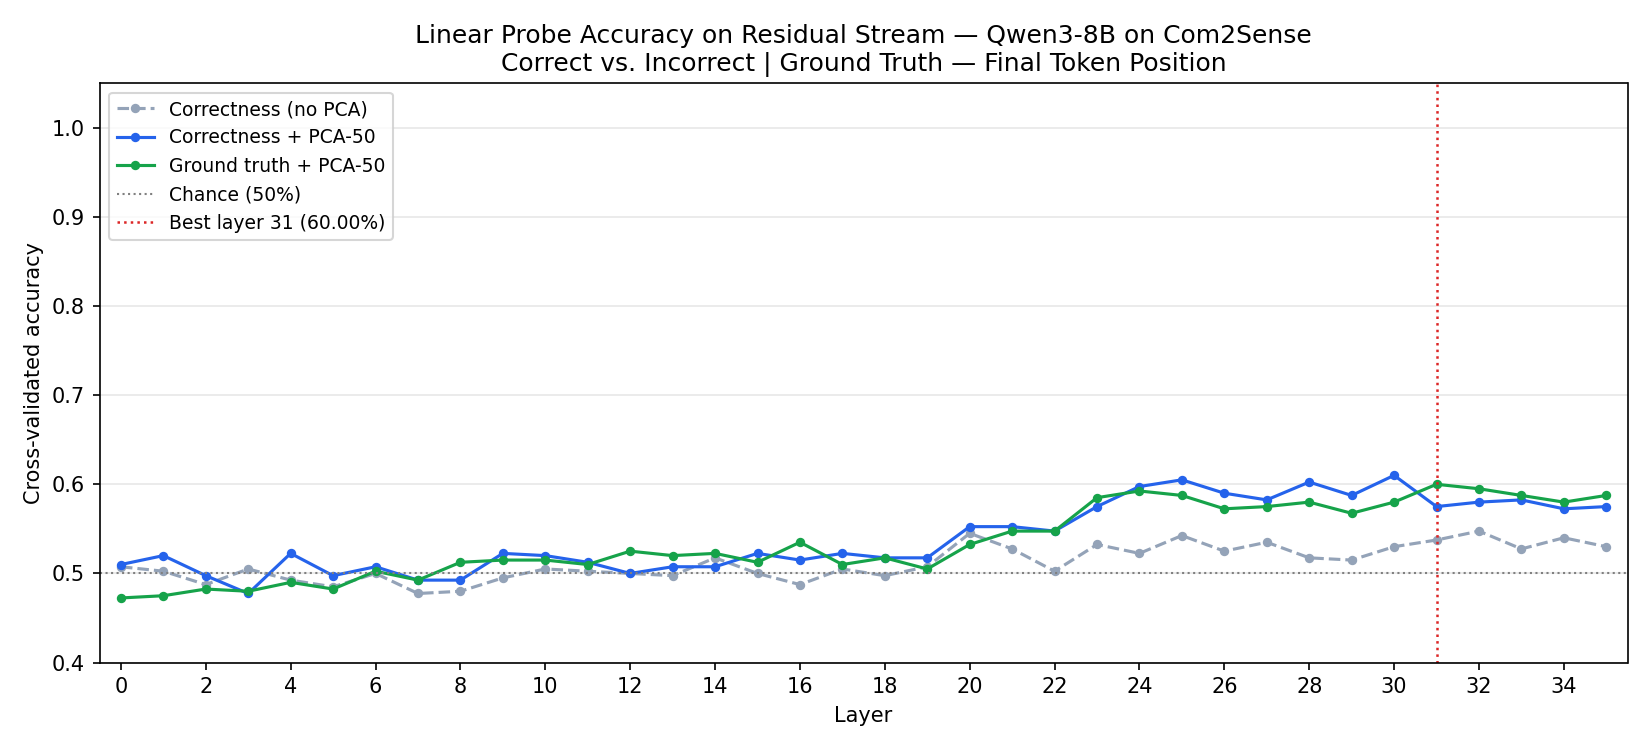
\includegraphics[width=0.9\linewidth]{reports/figures/probe_accuracy_curve.png}
\caption{Residual-stream probe accuracy across layers. The probe signal stays weak early and rises only in the latter half of the network.}
\label{fig:probe-curve}
\end{figure}

Because the phase-2 setup uses 4096-dimensional features with only 400 examples, the repository includes a follow-up L2 sweep to measure overfitting. That correction lowers the best PCA-based results slightly and raises the heavily regularized no-PCA result, producing a cleaner estimate of genuine signal.

\begin{table}[t]
\centering
\begin{tabular}{lccc}
\toprule
Probe & Best $C$ & Best layer & Best accuracy \\
\midrule
Correctness (no PCA) & 0.001 & 34 & 57.50\% \\
Correctness + PCA-50 & 0.01 & 23 & 58.75\% \\
Ground truth + PCA-50 & 0.01 & 32 & 59.25\% \\
\bottomrule
\end{tabular}
\caption{Regularization-corrected probe results from \texttt{artifacts/analysis/l2\_sweep\_results.json}.}
\label{tab:l2-sweep}
\end{table}

The corrected conclusion is that the residual stream carries only weak linear signal about commonsense truth. The practical ceiling is about 59\%, not 61\%, and correctness is not substantially easier to decode than ground truth after regularization. This weak separability already points away from a clean, robust internal representation of the correct answer.

\begin{figure}[t]
\centering
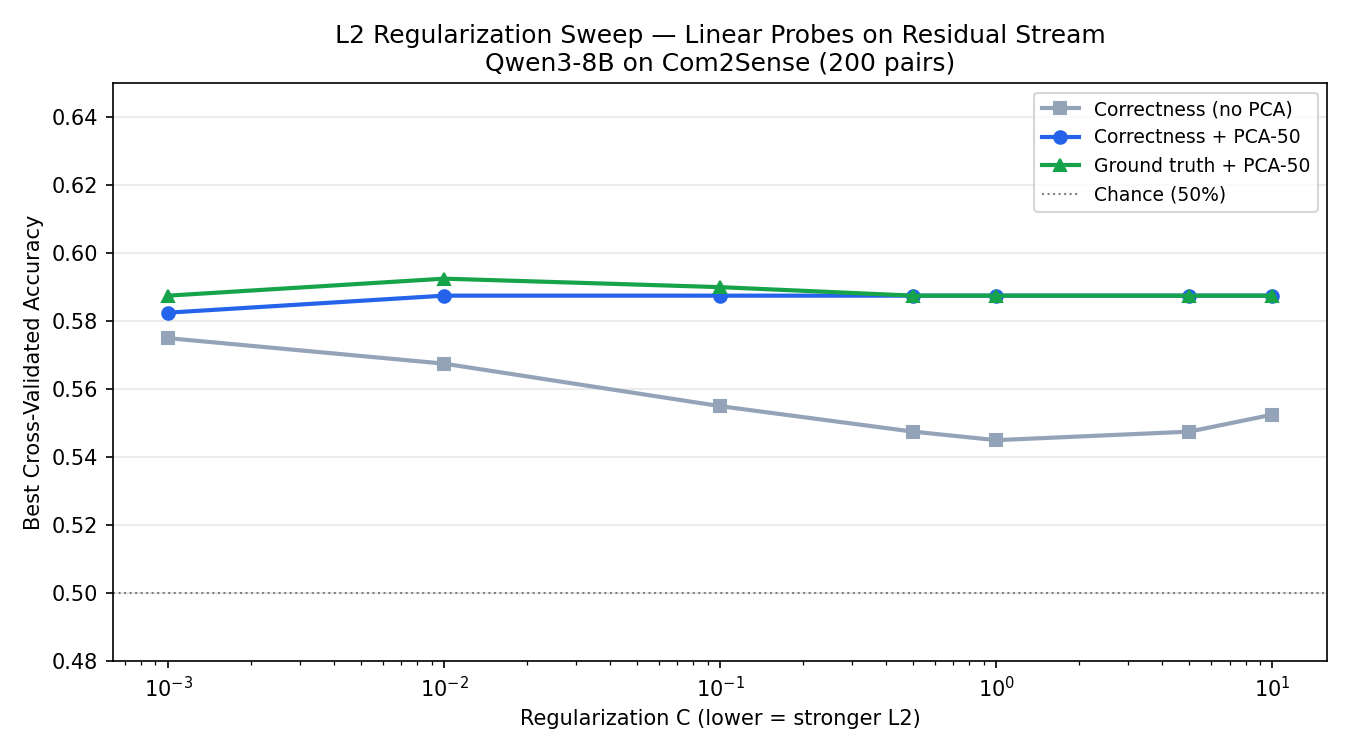
\includegraphics[width=0.85\linewidth]{reports/figures/l2_sweep_results.png}
\caption{L2 sweep results. PCA provides most of the regularization benefit, and the corrected probing ceiling remains near 59\%.}
\label{fig:l2-sweep}
\end{figure}

\section{Causal Intervention Results}

\subsection{Layer-level activation patching}

Residual-stream patching tests sufficiency: if a single layer contains the decisive computation, replacing that layer's final-token residual state in an incorrect example with the corresponding state from the correct paired example should often flip the answer.

That does not happen. Across layers 18--35, the flip rate is 0\% at every layer except layer 26, which produces exactly one flip out of 200 pairs (0.5\%). Mean logit changes are negative throughout, from $-0.006$ at layer 18 to $-0.355$ at layer 35. Patching the full residual stream generally makes the prediction worse rather than better.

\begin{figure}[t]
\centering
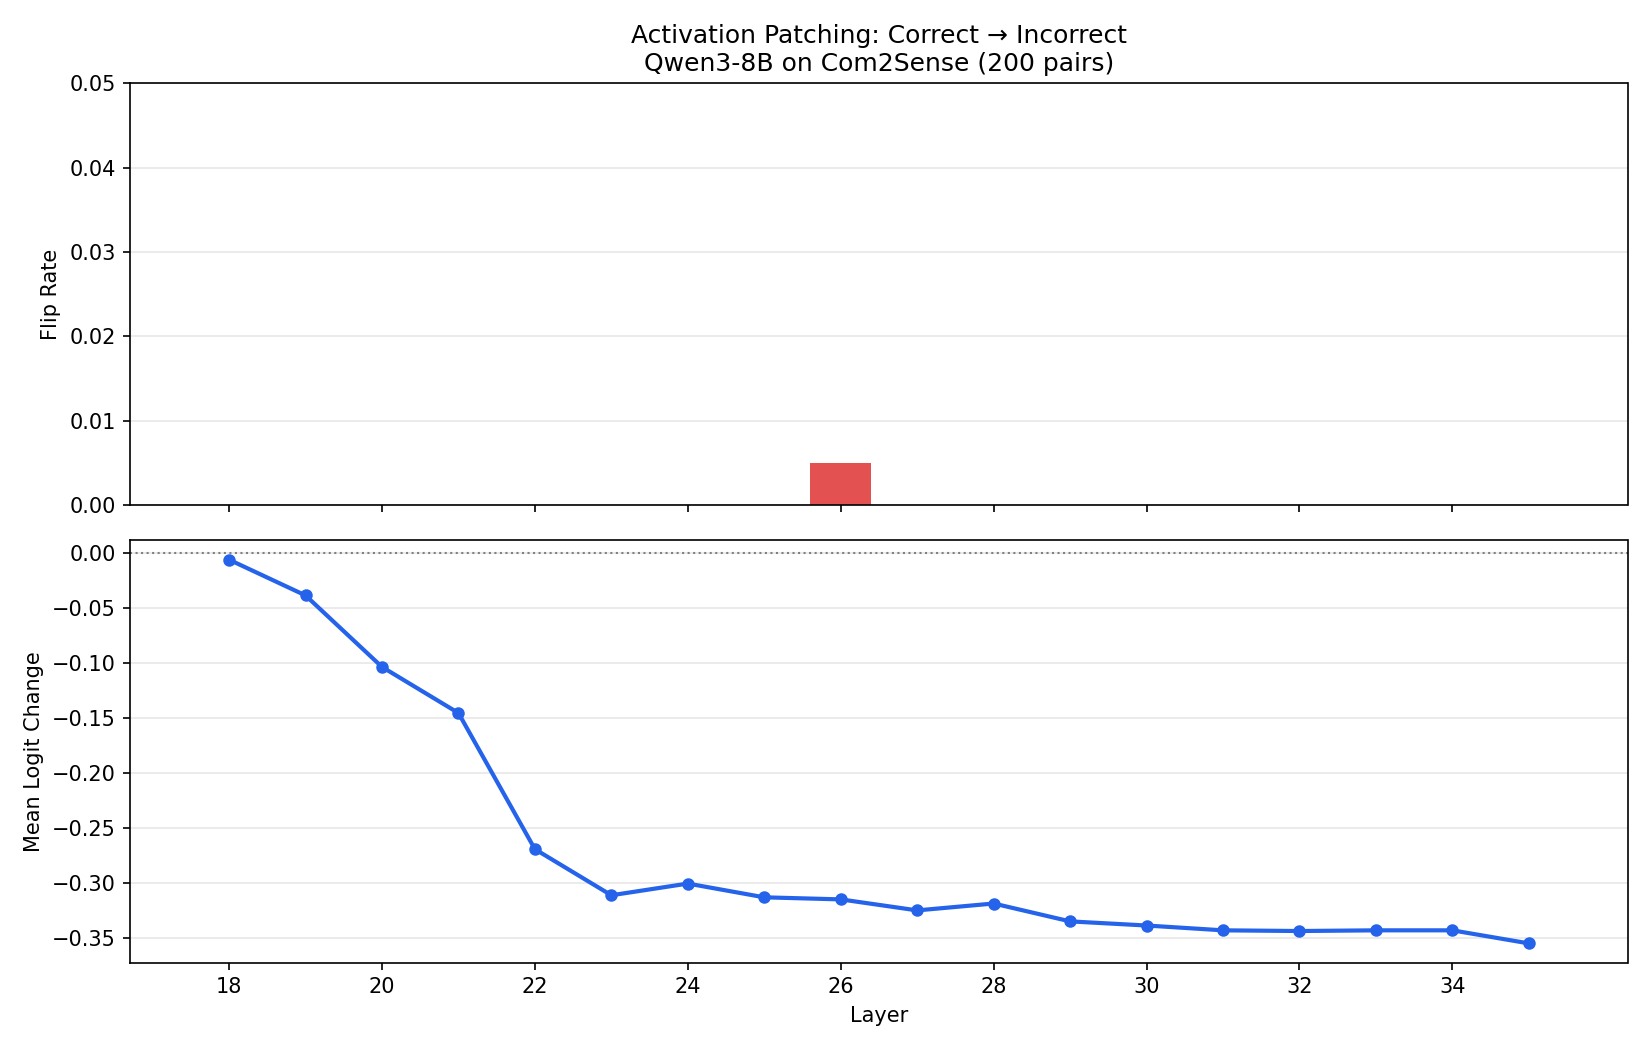
\includegraphics[width=0.9\linewidth]{reports/figures/patching_results.png}
\caption{Layer-level activation patching results. No layer is sufficient to reliably flip incorrect predictions.}
\label{fig:patching}
\end{figure}

\subsection{Head-level patching and head-level probing}

Head-level patching asks the same sufficiency question at finer granularity. The five target layers chosen from the patching phase were layers 26, 18, 19, 20, and 21. Across all 160 tested layer-head combinations, the flip rate is 0\%. The most influential head is L20.H8 with mean effect $-0.068$ and absolute mean effect 0.147, still tiny relative to the average wrong-answer gap of 2.534.

Head-level probing gives the complementary informational picture. The best single heads reach almost exactly the same accuracy as the full residual stream:

\begin{table}[t]
\centering
\begin{tabular}{lcc}
\toprule
Configuration & Best head & Accuracy \\
\midrule
Correctness, final token & L32.H20 & 59.50\% \\
Correctness, statement-end & L28.H11 & 58.25\% \\
Ground truth, final token & L34.H18 & 59.50\% \\
Ground truth, statement-end & L35.H23 & 59.25\% \\
\bottomrule
\end{tabular}
\caption{Best per-head probe results from \texttt{artifacts/analysis/head\_probe\_results.json}.}
\label{tab:head-probes}
\end{table}

This combination is important. No head is causally sufficient to fix the task, but many heads are similarly informative. The informative heads and the most causally influential heads do not coincide, which suggests that information presence and causal bottleneck structure are dissociated here.

\begin{figure}[t]
\centering
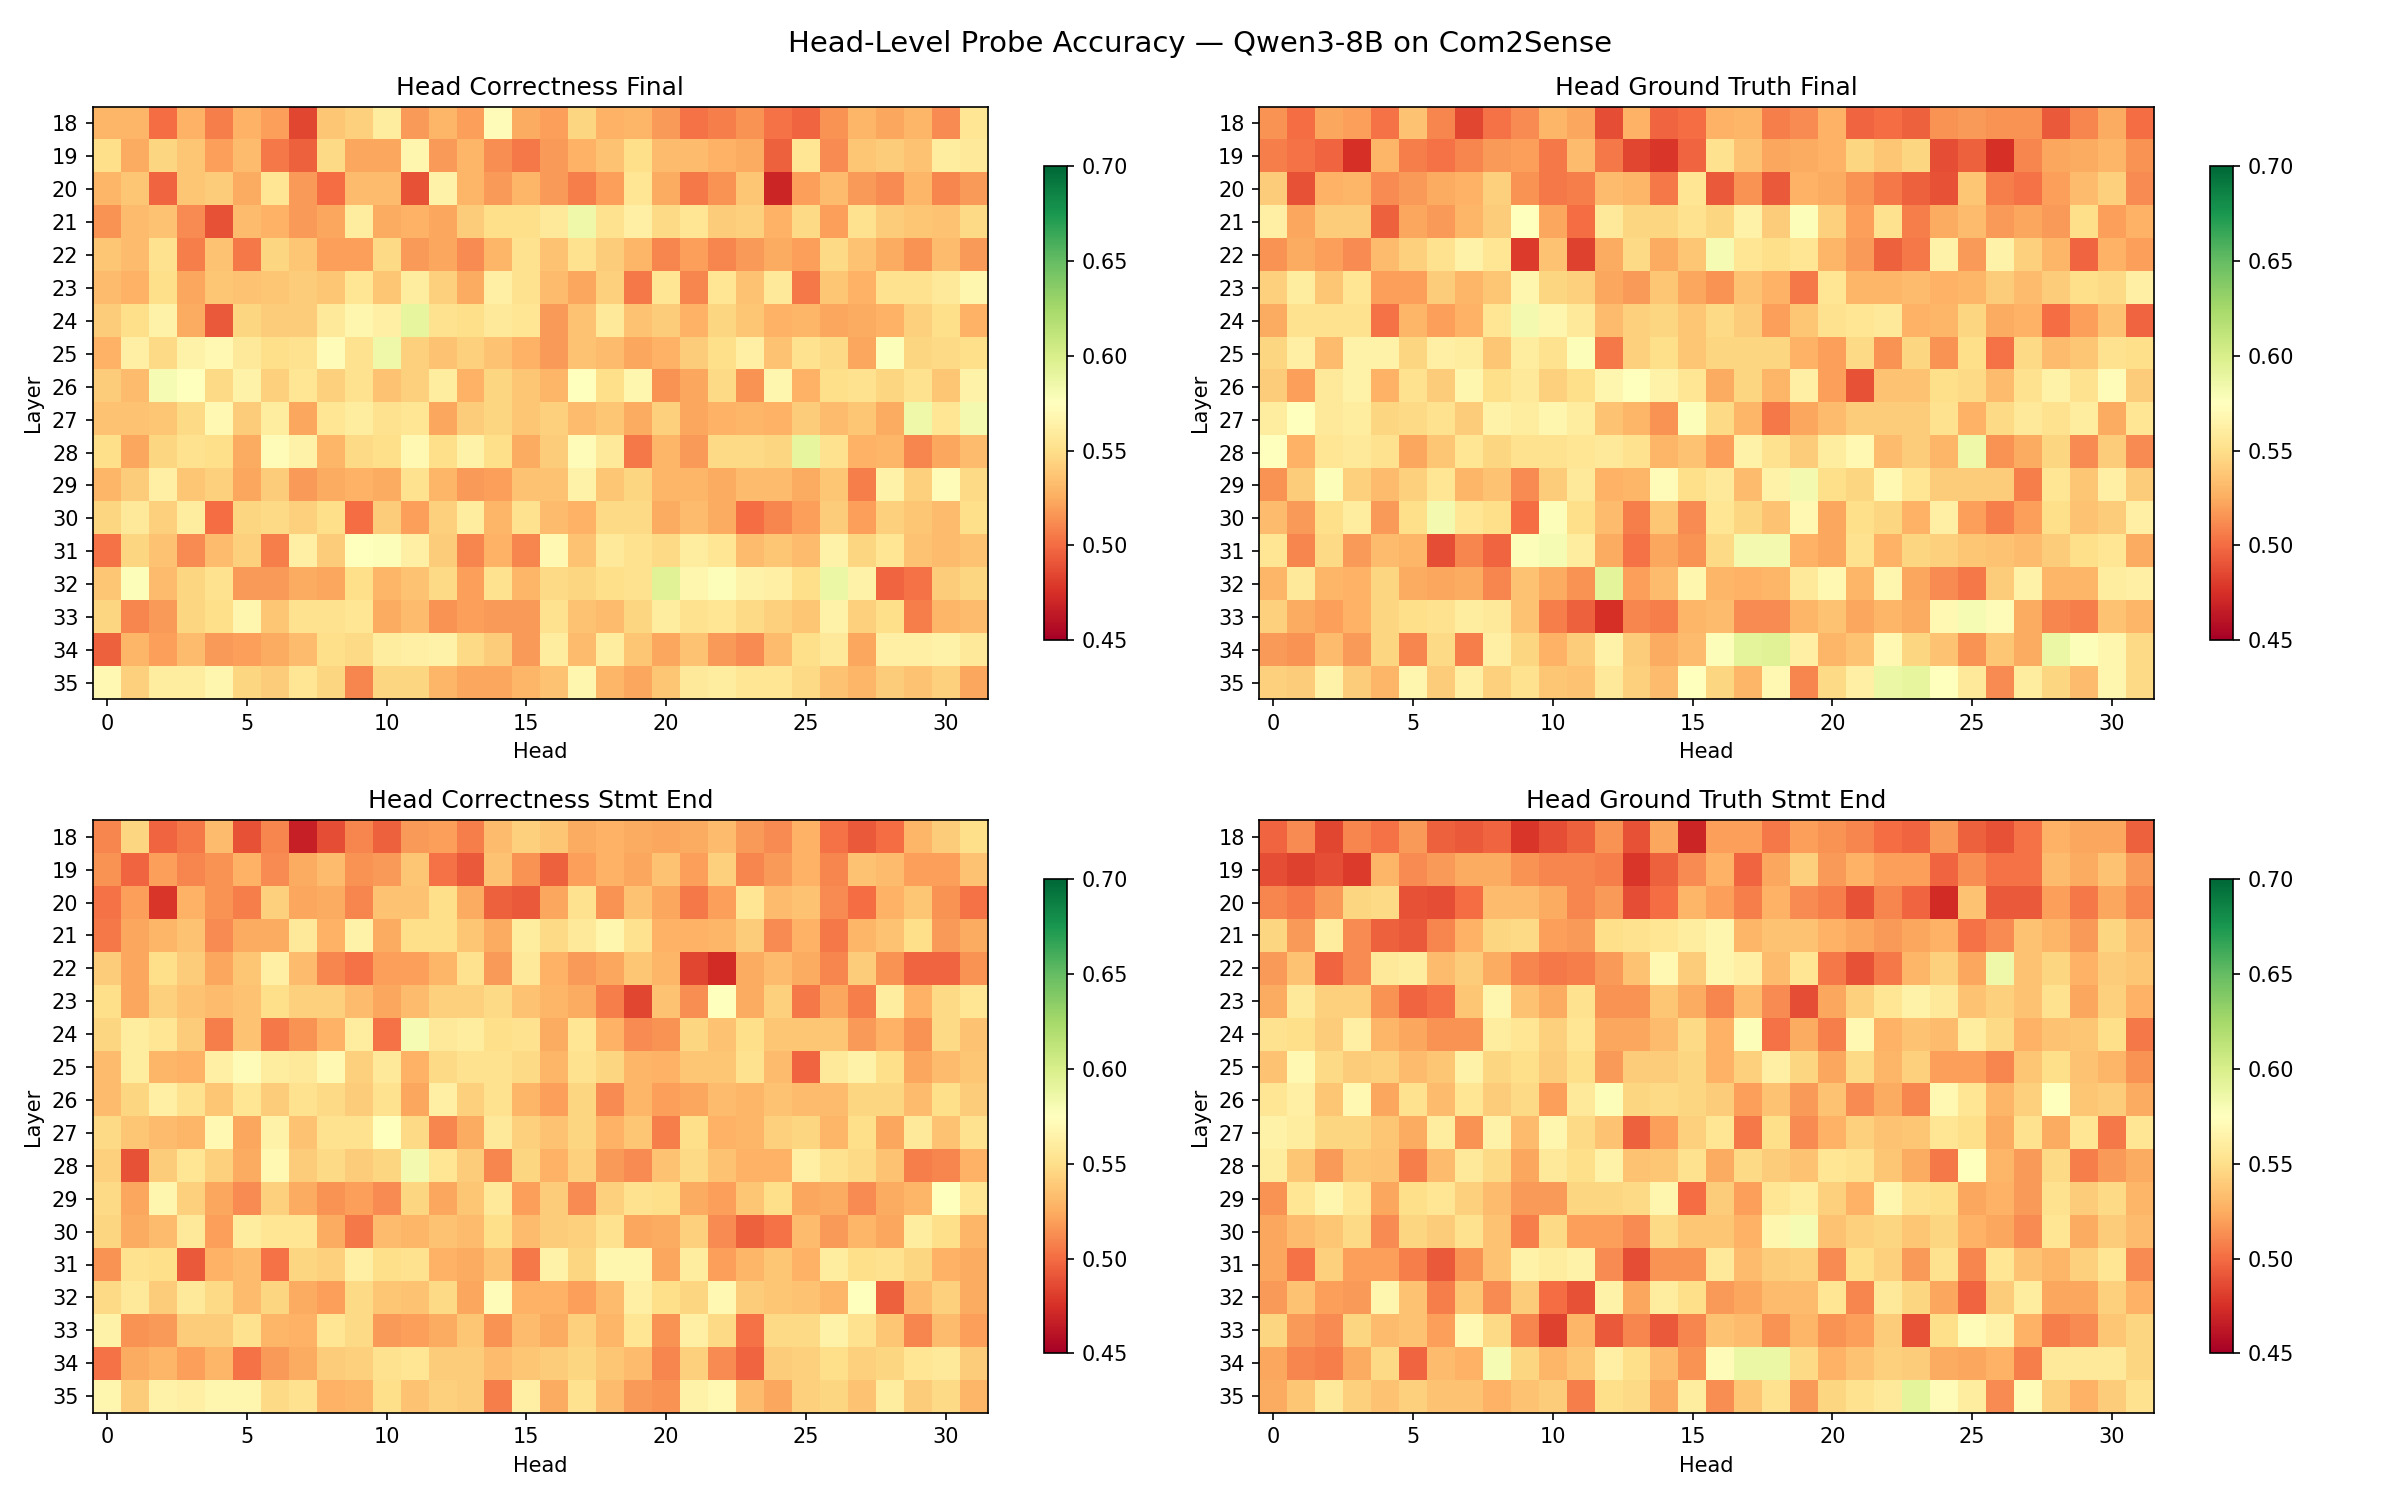
\includegraphics[width=0.92\linewidth]{reports/figures/head_probe_heatmap.png}
\caption{Head-level probe accuracy heatmap. Signal is weak and broadly distributed rather than concentrated in one standout head.}
\label{fig:head-heatmap}
\end{figure}

\subsection{Attention-vs-MLP decomposition}

The repository also decomposes layer patching into separate attention-output and MLP-output interventions. This avoids conflating the two sublayers inside \texttt{resid\_post}.

The result stays the same at the level that matters. Neither sublayer produces reliable flips. The strongest positive attention result is layer 25, with a 1.5\% flip rate and mean logit change $+0.163$. The strongest MLP result is layer 35, also with a 1.5\% flip rate and mean logit change $+0.133$. These are the best outcomes in the entire intervention study, but they are still far too small to support a localized-bottleneck interpretation.

\begin{figure}[t]
\centering
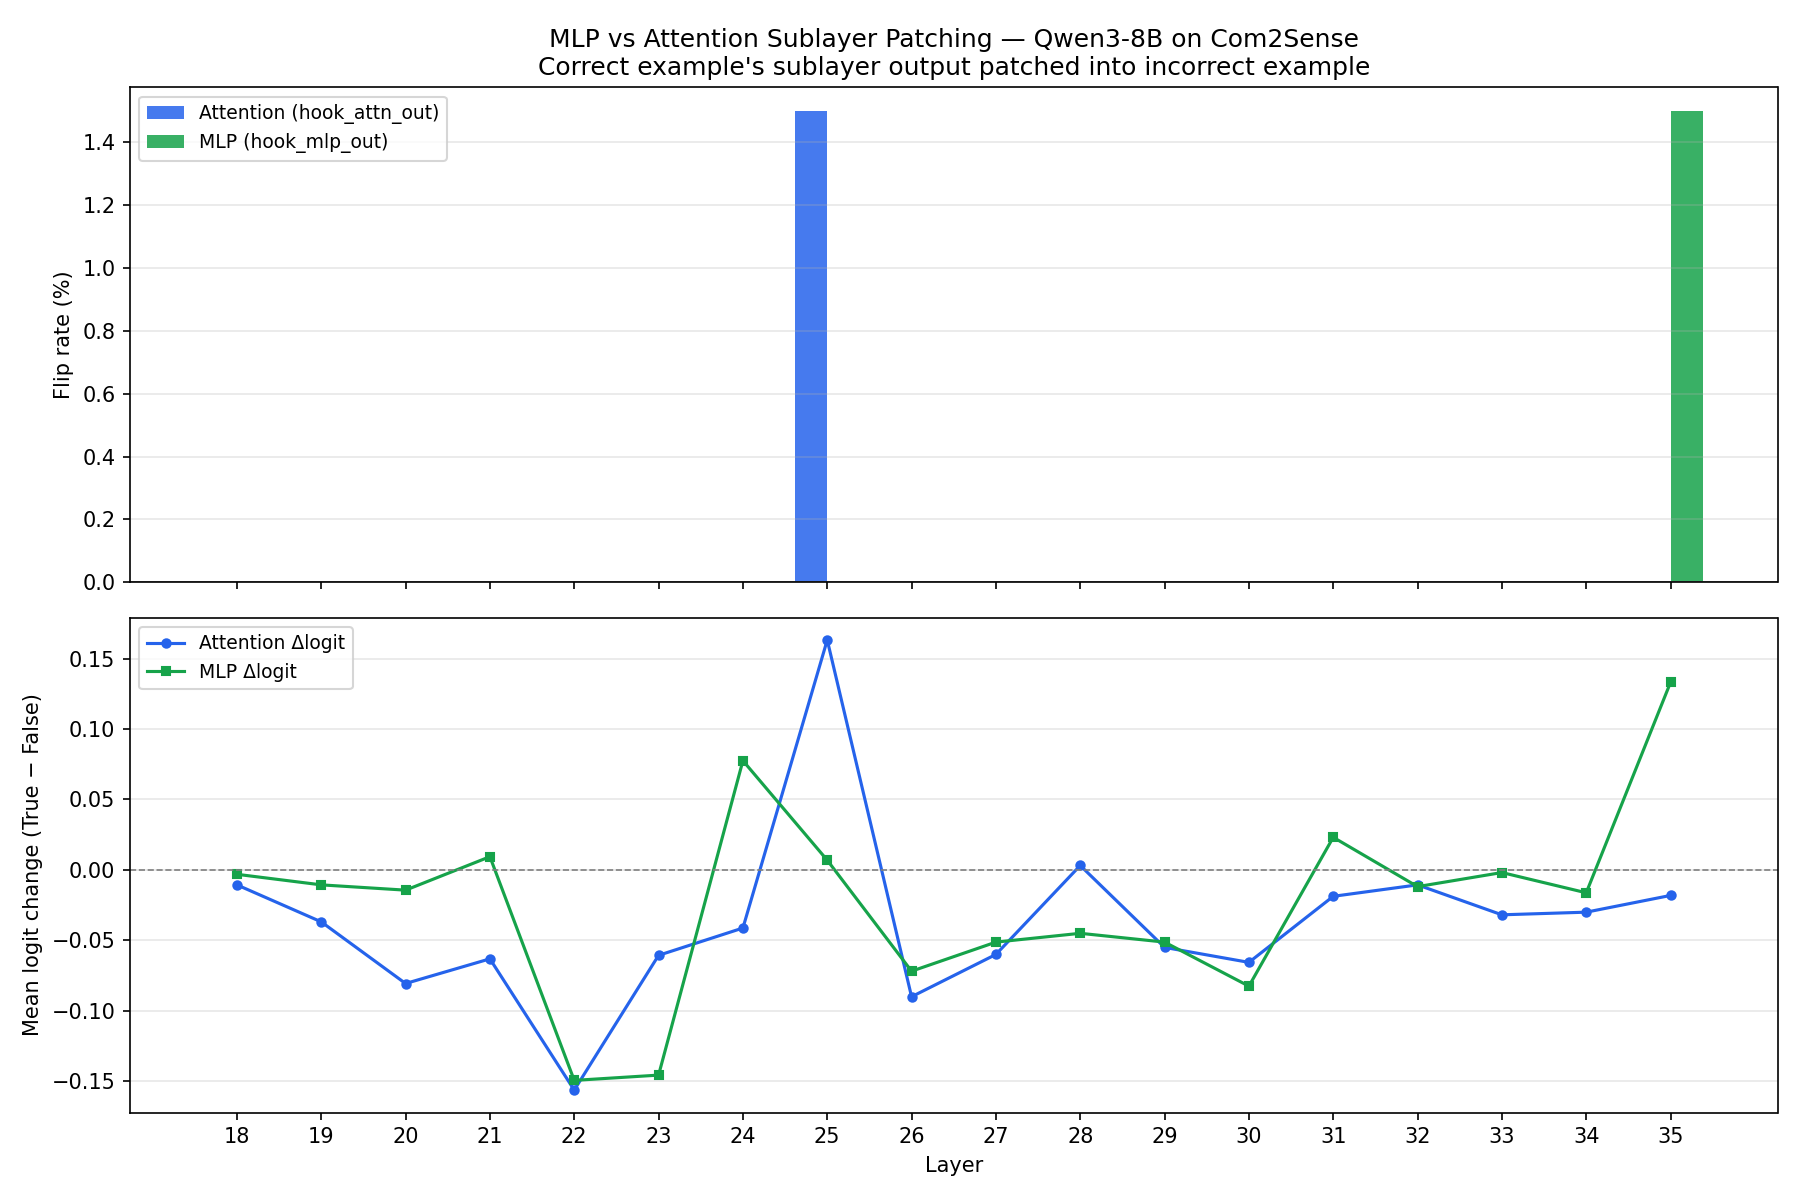
\includegraphics[width=0.9\linewidth]{reports/figures/mlp_attn_patching.png}
\caption{Attention-vs-MLP sublayer patching. Neither sublayer type shows a reliable causal bottleneck.}
\label{fig:mlp-attn}
\end{figure}

\subsection{Mean-ablation}

Mean-ablation tests necessity rather than sufficiency by removing candidate head contributions from examples the model originally answers correctly. If the patching and probing candidates were truly essential, ablation should break a meaningful number of correct predictions.

It does not. Across 17 target heads, the maximum flip rate is only 1.0\% (L26.H25, 2 flips out of 200). The largest absolute mean logit change is 0.028 for L18.H6, which is negligible. Heads that looked best under probing and heads that looked strongest under patching are both weak under ablation. Together with the patching results, this strongly supports the claim that no single head is either necessary or sufficient for these commonsense judgments.

\begin{figure}[t]
\centering
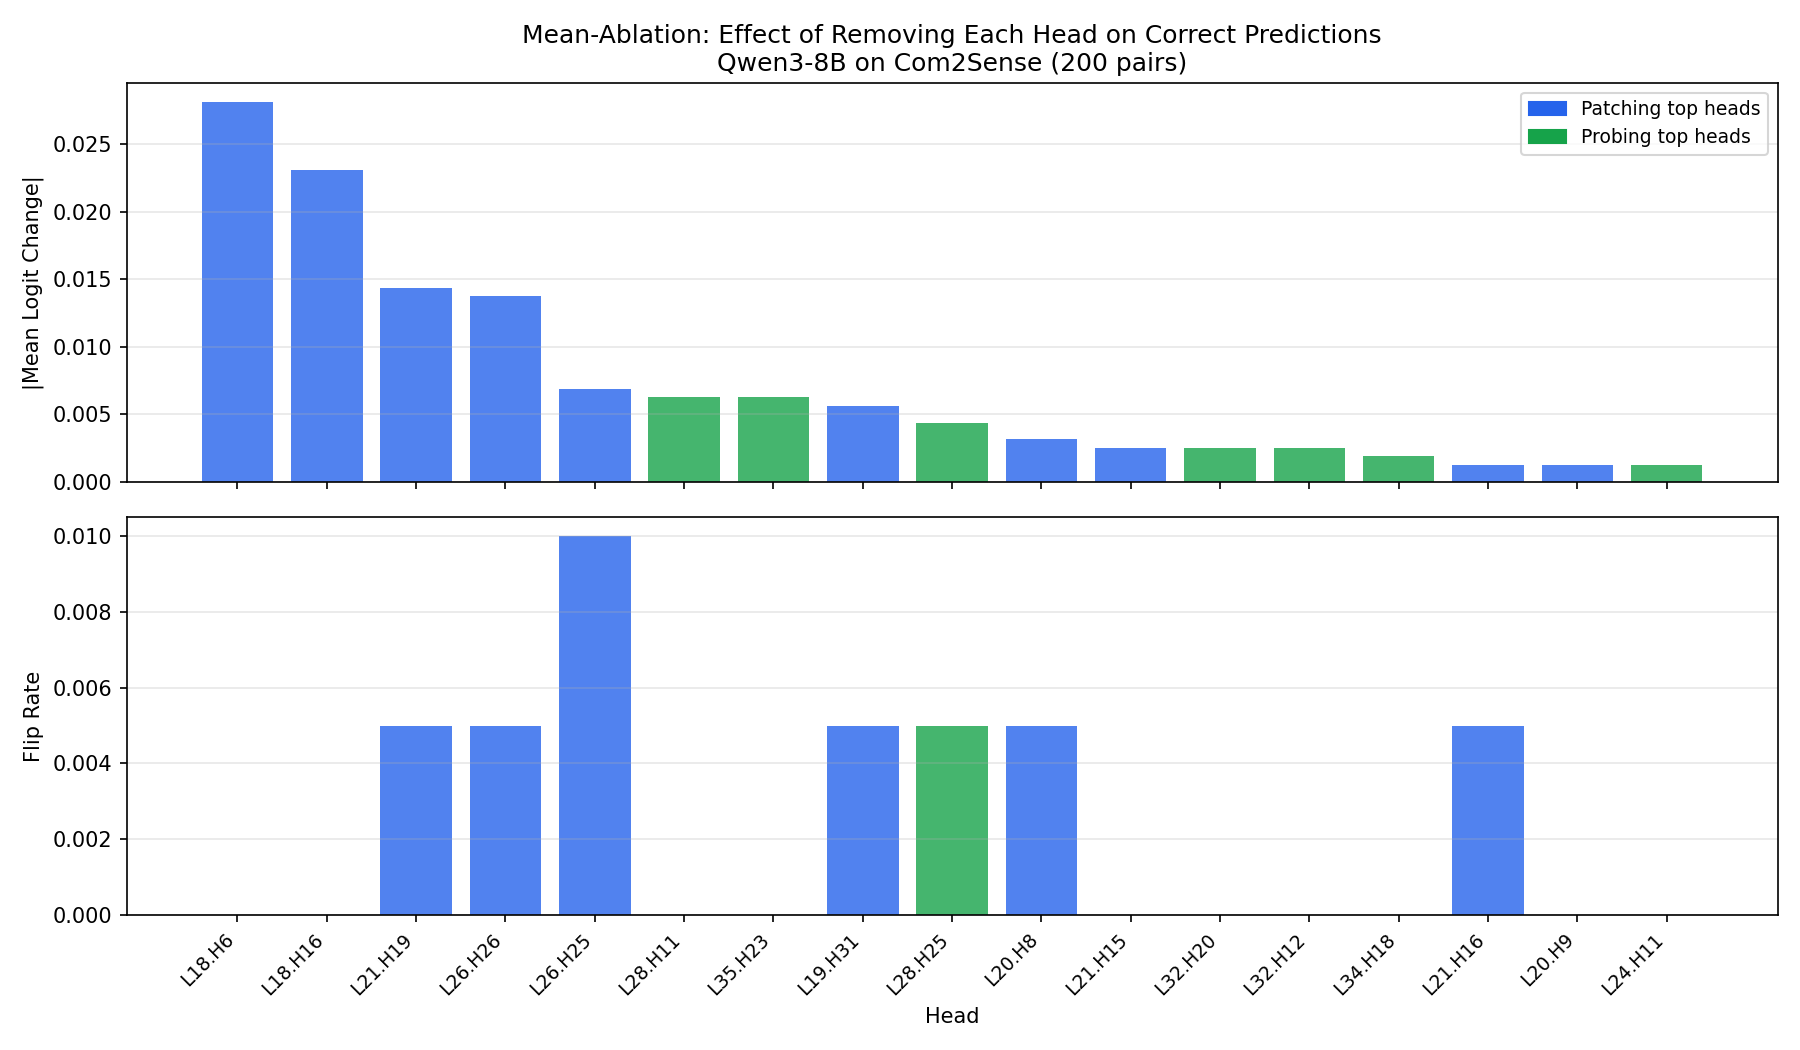
\includegraphics[width=0.85\linewidth]{reports/figures/ablation_results.png}
\caption{Mean-ablation on candidate heads. Even targeted removal of the strongest heads has minimal behavioral effect.}
\label{fig:ablation}
\end{figure}

\section{Logit Lens and Failure Timing}

The logit-lens analysis changes the temporal interpretation of the project. Instead of asking whether truth is linearly decodable at a layer, logit lens asks what answer the model is already moving toward when each layer's residual stream is projected through the final unembedding.

This produces a more nuanced answer than the original ``late-only failure'' story. Incorrect examples are often biased toward the wrong answer almost immediately: 153 of the 200 incorrect examples are already on the wrong side at layer 0, and the mean first-wrong layer is 1.61. But the wrong answer usually does not become stable until much later: the mean stable-wrong layer is 19.885, while the mean stable-correct layer for correct examples is 20.235.

\begin{table}[t]
\centering
\begin{tabular}{lc}
\toprule
Metric & Value \\
\midrule
First strong divergence layer & 0 \\
Mean incorrect first-wrong layer & 1.61 \\
Mean incorrect stable-wrong layer & 19.885 \\
Mean correct stable-correct layer & 20.235 \\
Mean final signed gap, correct & +2.8088 \\
Mean final signed gap, incorrect & -2.5319 \\
\bottomrule
\end{tabular}
\caption{Aggregate logit-lens trajectory statistics from \texttt{results\_download/logit\_lens/logit\_lens\_summary.json}.}
\label{tab:logit-lens}
\end{table}

The layer trajectories are also non-monotonic. Correct and incorrect examples separate early, partially reverse in mid layers, and then separate again strongly in the late-middle and late network. That pattern matches a distributed multi-stage computation better than a single write-once decision circuit.

\begin{figure}[t]
\centering
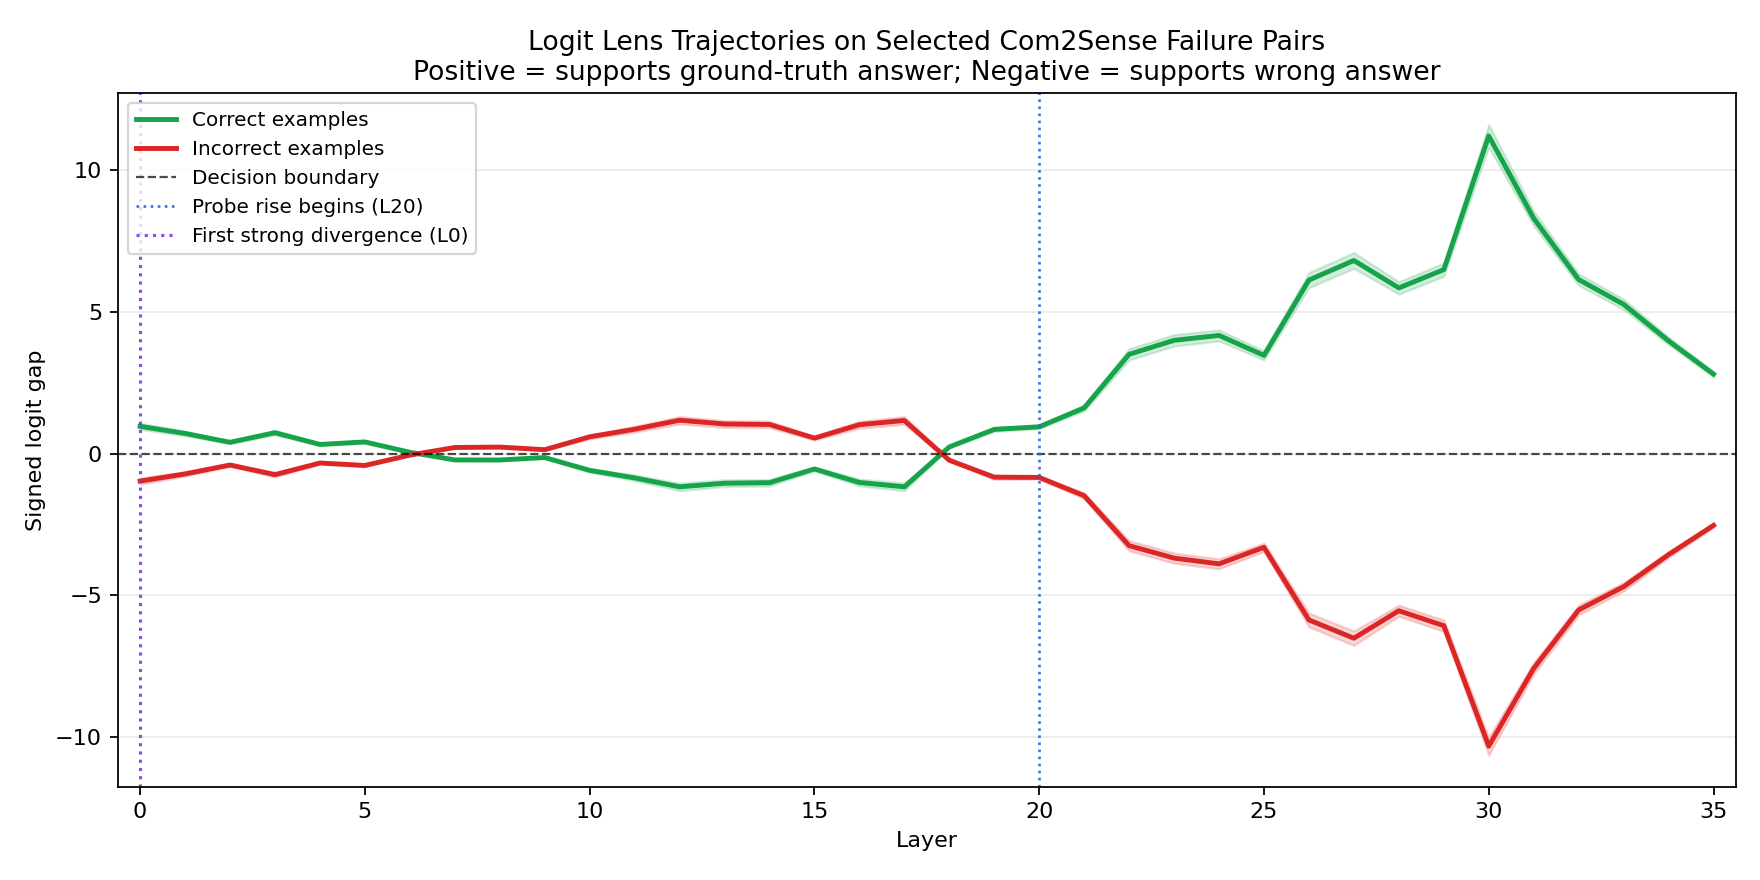
\includegraphics[width=0.9\linewidth]{reports/figures/logit_lens_trajectories.png}
\caption{Logit-lens trajectories for correct and incorrect examples. The preference for the final answer is dynamic rather than monotonic.}
\label{fig:logit-lens}
\end{figure}

Logit lens therefore refines the earlier inference. The failures are not purely late-onset, because many incorrect examples are already tilted toward the wrong answer very early. But they are not simply wrong from the start either, because the decisive commitment usually arrives around layer 20. The most accurate description is \emph{early bias plus late consolidation}.

\section{Discussion}

Across all phases, the same structural conclusion keeps reappearing.

\textbf{Localized or distributed?} Distributed. Residual patching finds no sufficient layer. Head patching finds no sufficient head. Mean-ablation finds no necessary head. Head-level probing shows that multiple heads carry similarly weak signal, rather than one dominant circuit.

\textbf{Architectural or representational?} The evidence points most strongly to a representational problem. The model is not at chance: probes and logit lens both reveal nontrivial signal. But that signal is weak, diffuse, and unstable, which means the architecture can in principle express the task while failing to build a strong enough internal representation to solve it robustly.

\textbf{Early or late failure?} The updated answer is neither ``purely early'' nor ``purely late.'' The project started with a late-inference interpretation because linearly separable probe signal mostly appears from layer 20 onward. Logit lens revises that story: wrong-answer bias is often present from the earliest measured layer, but the final answer typically becomes stable around layer 20. The failure process is therefore distributed in time as well as in space.

\textbf{Why the patching signal is so weak.} The repository's decomposition experiments suggest two reasons. First, swapping entire states between different paired sentences creates a distributional mismatch, which explains why \texttt{resid\_post} patching often degrades performance. Second, even cleaner attention-only and MLP-only interventions remain too small to recover the answer, which indicates that the underlying signal is simply not concentrated enough for surgical repair.

\section{Conclusion}

The current version of the repository supports a clear headline result: commonsense failures in Qwen3-8B on Com2Sense are distributed, weakly represented, and not recoverable through single-component intervention. The model is behaviorally competent enough to show structured successes and failures, but the internal evidence for the correct answer peaks at only about 59\% under controlled probing, and neither layer- nor head-level intervention identifies a compact causal circuit.

The most defensible end-state claim is therefore:

\begin{quote}
Commonsense failure in this setting is best described as a distributed representational deficit with early wrong-answer bias and late consolidation, rather than a localized bottleneck at one layer, one head, or one sublayer.
\end{quote}

Two follow-ups are especially well motivated by the current artifact set: a failure-direction-specific logit-lens split to test whether the early bias is specifically a false-bias, and position-sensitive logit lens to compare statement-end and final-token trajectories directly.

\end{document}
